\documentclass[10pt, a4paper, oneside]{article}
\usepackage[utf8]{inputenc}
\usepackage[english]{babel}
\usepackage{graphicx}
\usepackage{amsmath}
\usepackage{amssymb}
\usepackage{amsthm}
\usepackage{epstopdf}
\usepackage{vhistory}
\usepackage{framed}
\usepackage{hyperref}
\usepackage[left=30mm, right=30mm]{geometry}

\setlength{\parskip}{11pt}

%% Están definidos los conjuntos típicos.
\newcommand{\N}{\ensuremath{\mathbb{N}}}
\newcommand{\Z}{\ensuremath{\mathbb{Z}}}
\newcommand{\Q}{\ensuremath{\mathbb{Q}}}
\newcommand{\R}{\ensuremath{\mathbb{R}}}
\newcommand{\C}{\ensuremath{\mathbb{C}}}

%% rme, rmi e Id son el número e, el número imaginario i y la identidad respectivamente. Poned ds antes de una expresión
%% cuando salga mal (en las fracciones y cosas parecidas)
\def\ds{\displaystyle}
\def\rme{\mathrm{e}}
\def\rmi{\mathrm{i}}
\def\Id{\mathrm{Id}}
\def\resposta{\bullet\bullet\bullet\bullet\bullet\bullet}


%% Los tipos de enunciados. Los he copiado del examen de numérico, así que ponedlos bien
\newtheorem{thm}{Theorem}[section]
\newtheorem{main_thm}[thm]{Main Theorem}
\newtheorem{cor}[thm]{Corollary}
\newtheorem{lem}[thm]{Lemma}
\newtheorem{prop}[thm]{Proposition}
\newtheorem{defn}[thm]{Definition}
\newtheorem{rem}[thm]{Comment}
\newtheorem{prob}[thm]{Exercici}

\newtheorem*{remark}{Remark}
\newtheorem*{definition}{Definition}
\newtheorem*{example}{Example}

%% Si vais a escribir muchas veces algo con un cierto formato, definidlo aqui
\newcommand{\taylor}{\textsf{Taylor}}
\newcommand{\HH}{\emph{Hénon-Heiles}}

%% Si una palabra se parte mal al final de linea la poneis aqui
\hyphenation{Bar-ce-lo-na}


%% Ejemplo de como hacer una tabla.

%\begin{tabular}{|r|c|c|}
%\hline
%$n$	&nº bits (estándar)	&nº bits (\emph{sp. triplet})\\
%\hline
%10   	  &  6400       	& 3040\\
%\hline
%50   	  & 160000    	& 78400\\
%\hline
%100 	  & 640000    	& 314320\\
%\hline
%200 	  & 2560000  	& 1262320\\
%\hline
%400 	  & 10240000	&5043680\\
%\hline
%650 	  & 27040000	&13282720\\
%\hline
%1000 	  & 64000000	&31479040\\
%\hline
%\end{tabular}


%% Ejemplo de como hacer una figura

%\begin{figure}[ht]
%\centering
%\includegraphics[width=6cm,angle=-90]{exemple.eps}
%\caption{Corba de continuaci\'o d'$u_2$ com a funci\'o de $\lambda$.}
%\label{fig:etiqueta}
%\end{figure} 

%% se puede hacer \input{archivo.tex} en lugar de \includegraphics

%% Y de como hacerle referencia

% bla bla bla en la Figura~\ref{fig:etiqueta}

% math stuff
\newcommand{\Expect}{\ensuremath{{\rm I\kern-.3em E}}}
\newcommand{\Var}{\ensuremath{\mathrm{Var}}}
\newcommand{\Cov}{\ensuremath{\mathrm{Cov}}}


% random
\makeatletter
\newcommand{\raisemath}[1]{\mathpalette{\raisem@th{#1}}}
\newcommand{\raisem@th}[3]{\raisebox{#1}{$#2#3$}}
\makeatother

\newcommand{\function}[5]{\begin{split} #1\colon #2 &\to #3 \\ #4 &\mapsto #5\end{split}}

% xanadu but random
\newcommand{\atm}{\ensuremath{\mathit{ATM}}}
\newcommand{\somconst}{\ensuremath{k_{\mathit{som}}}}

% sets
\newcommand{\expiries}{\ensuremath{\mathbb{E}}}
\newcommand{\options}{\ensuremath{\mathbb{O}}}
\newcommand{\puts}{\ensuremath{\mathbb{P}}}
\newcommand{\calls}{\ensuremath{\mathbb{C}}}
\newcommand{\mfuture}{\ensuremath{\mathcal{F}}}
\newcommand{\future}{\ensuremath{\mathrm{F}}}
\newcommand{\rolls}{\ensuremath{\circlearrowleft}}
\newcommand{\total}{\ensuremath{\mathbb{T}}}
\newcommand{\offsets}{\ensuremath{\Xi}}
\newcommand{\scenarios}{\ensuremath{\mathbb{S}}}
\newcommand{\moneynessset}{\ensuremath{\mathcal{X}}}
\newcommand{\params}{\ensuremath{\mho}}

% values
\newcommand{\sdelta}{\ensuremath{\tilde{\delta}}}
\newcommand{\sgamma}{\ensuremath{\tilde{\Gamma}}}
\newcommand{\stheta}{\ensuremath{\tilde{\theta}}}
\newcommand{\cstheta}{\ensuremath{\widetilde{\cash\theta}}}
\newcommand{\vega}{\ensuremath{\nu}}
\newcommand{\volatility}{\ensuremath{\sigma}}
\newcommand{\basevol}{\ensuremath{{\volatility_{\!\raisemath{-2pt}{B}}}}}
\newcommand{\vegabv}{\ensuremath{{\vega_\basevol}}}
\newcommand{\slope}{\ensuremath{m}}
\newcommand{\vegaslo}{\ensuremath{{\vega_\slope}}}
\newcommand{\atmvega}{\ensuremath{{\vega_{\!\raisemath{-2pt}{\atm(e)}}}}}
\newcommand{\atmvegabv}{\ensuremath{{\vegabv_{\!\raisemath{-2pt}{\atm(e)}}}}}
\newcommand{\pos}{\ensuremath{p}}
\newcommand{\price}{\ensuremath{\upsilon}}
\newcommand{\yte}{\ensuremath{\mathcal{Y}}}

\newcommand{\cash}{\ensuremath{\mathdollar}}
\newcommand{\risk}{\ensuremath{\mathcal{R}}}

% perceived risk and cash
\newcommand{\pcash}{\ensuremath{\overline{\cash}}}
\newcommand{\prisk}{\ensuremath{\overline{\risk}}}

% normalized vega for base volatility
\newcommand{\nvegabv}{\ensuremath{\overline{\vegabv}}}
\newcommand{\pnvegabv}{\ensuremath{\dot{\overline{\vegabv}}}}

% propagated vega
\newcommand{\pvega}{\ensuremath{\hat{\vega}}}
\newcommand{\pvegam}{\ensuremath{{\pvega_\moneyness}}}
\newcommand{\pvegad}{\ensuremath{{\pvega_\delta}}}

% final vega
\newcommand{\fvega}{\ensuremath{\breve{\vega}}}
\newcommand{\fvegam}{\ensuremath{{\fvega_\moneyness}}}
\newcommand{\fvegad}{\ensuremath{{\fvega_\delta}}}

% normalized vega
\newcommand{\nvega}{\ensuremath{\dot{\vega}}}
\newcommand{\nvegam}{\ensuremath{{\nvega_\moneyness}}}
\newcommand{\nvegad}{\ensuremath{{\nvega_\delta}}}

\newcommand{\offsetbs}{\ensuremath{\xi^{\pm}}}

% functions
\newcommand{\moneyness}{\ensuremath{\chi}}
\newcommand{\VoV}{\ensuremath{\mathit{Vo\!V}}}

% settings
\newcommand{\target}{\ensuremath{\mathit{tg}}}
\newcommand{\widen}{\ensuremath{\mathit{widen}}}
\newcommand{\skw}{\ensuremath{\mathit{skew}}}
\newcommand{\offset}{\ensuremath{\mathit{offset}}}

% formulas
\newcommand{\skewunits}[3]{\ensuremath{\frac{{#1}\mp{#2}-\target}{{#3}}}}
\newcommand{\offsetformula}[4]{{\begin{align*}\offsetbs_{#4}=\pm\left|\skewunits{#1}{#2}{#3}\cdot\widen\cdot{#2}\right| \pm \left|\offset\cdot{#2}\right| - \skewunits{#1}{#2}{#3}\cdot\skw\cdot{#2}.\end{align*}}}
\newcommand{\offsetformulacomma}[4]{{\begin{align*}\offsetbs_{#4}=\pm\left|\skewunits{#1}{#2}{#3}\cdot\widen\cdot{#2}\right| \pm \left|\offset\cdot{#2}\right| - \skewunits{#1}{#2}{#3}\cdot\skw\cdot{#2},\end{align*}}}

\title{Exercise set \#1. MVA: Basic multivariate calculations in R}
\author{Laura Santulario Verdú  \\ Eudald Romo Grau}

\begin{document}

\maketitle
\iffalse
\begin{versionhistory}
  \renewcommand \vhAuthorColWidth{.9\hsize}
  \renewcommand \vhChangeColWidth{1\hsize}
  
  \vhEntry{1.0}{2016.11.30}{\'Angel Garc\'ia G\'omez}{Created document and added first specifications for multiple expiries.}
  \vhEntry{1.1}{2016.12.20}{\'Angel Garc\'ia G\'omez}{Fixed errors in formulae and added cash skew theta.}
  \vhEntry{1.2}{2017.01.03}{\'Angel Garc\'ia G\'omez}{Updated vega offsets.}
  \vhEntry{1.3}{2017.02.01}{\'Angel Garc\'ia G\'omez}{Add offsets for the parameters movements.}
  \vhEntry{1.4}{2017.09.19}{\'Angel Garc\'ia G\'omez}{Add trade size chapter.}
  \vhEntry{1.5}{2018.01.16}{\'Angel Garc\'ia G\'omez}{Update cash skew theta offset. Add gamma and vega of expiry offsets.}
  \vhEntry{1.6}{2018.01.17}{\'Angel Garc\'ia G\'omez}{Update net option value offsets: total cash and perceived cash.}
  
\end{versionhistory}
\fi

\pagebreak

\section{Calculate the mean vector of the 6 numerical values.}

\vspace{5mm}
\begin{figure}[h!]\centering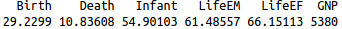
\includegraphics[scale=0.6]{pov_mean.png}\caption{Mean of each of the numerical values of the provided data.}\label{mean}\end{figure}
\vspace{5mm}

\section{Compute the centered data matrix.}

\vspace{5mm}
\begin{figure}[h!]\centering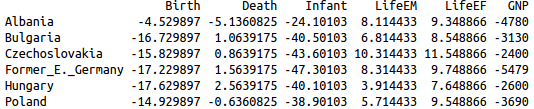
\includegraphics[scale=0.6]{pov_centered.png}\caption{Mean of each of the numerical values of the provided data.}\label{mean}\end{figure}
\vspace{5mm}

\section{Compute the variance-covariance matrix of the data.}

\vspace{5mm}
\begin{figure}[h!]\centering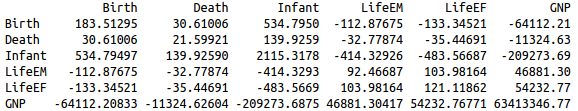
\includegraphics[scale=0.6]{pov_cov.png}\caption{Mean of each of the numerical values of the provided data.}\label{mean}\end{figure}
\vspace{5mm}

\pagebreak

\section{Compute the correlation matrix. Which variables show strong linear association?}

\vspace{5mm}
\begin{figure}[h!]\centering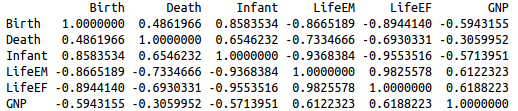
\includegraphics[scale=0.6]{pov_cor.png}\caption{Mean of each of the numerical values of the provided data.}\label{pov_cor}\end{figure}
\vspace{5mm}

The pair of variables with highest direct linear association is LifeEM-LifeEf and, on a lesser degree, Birth-Infant. The stronger inverse linear associations are between Birth/Infant and LifeEM/LifeEF (Birth-LifeEM, Birth-LifeEF, Infant-LifeEM, Infant-LifeEF).

\section{Compute the matrix of standardized variables.}

\vspace{5mm}
\begin{figure}[h!]\centering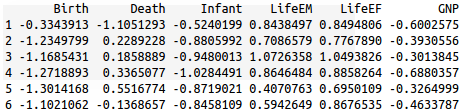
\includegraphics[scale=0.6]{poverty_standardized.png}\caption{Mean of each of the numerical values of the provided data.}\label{mean}\end{figure}
\vspace{5mm}

\section{Compute the variance-covariance matrix of standardized variables. What do you observe?}

The Variance-Covariance matrix of standardized data corresponds with the correlation matrix, as it can be seen in Fig. \ref{pov_cor} and \ref{sd_cov}

\vspace{5mm}
\begin{figure}[h!]\centering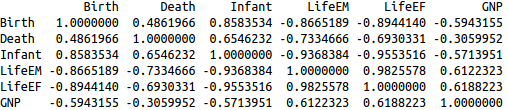
\includegraphics[scale=0.6]{pov_sd_cov.png}\caption{Mean of each of the numerical values of the provided data.}\label{sd_cov}\end{figure}
\vspace{5mm}

\section{Compute the matrix of Euclidean distances between the individuals, using the original data matrix. Which variable(s) contribute(s) most to the Euclidean distances? What could you do to reduce its/their influence?}

The variables with highest variance contribute the most to the Euclidean distance. As can be seen in Fig \ref{pov_sd}, GNP has the highest standard deviation (hence highest variance) and it can be seen 

\vspace{5mm}
\begin{figure}[h!]\centering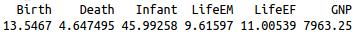
\includegraphics[scale=0.6]{pov_sd.png}\caption{Standard deviation of each of the numerical values of the provided data.}\label{pov_sd}\end{figure}
\vspace{5mm}

\vspace{5mm}
\begin{figure}[h!]\centering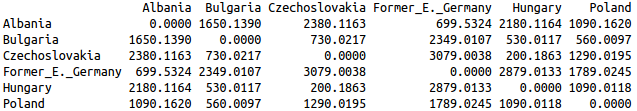
\includegraphics[scale=0.6]{pov_eucl_dist.png}\caption{Mean of each of the numerical values of the provided data.}\label{mean}\end{figure}
\vspace{5mm}

\pagebreak

\section{Compute the matrix of Mahalanobis distances between the individuals.}

\vspace{5mm}
\begin{figure}[h!]\centering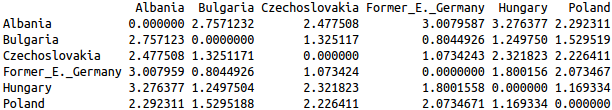
\includegraphics[scale=0.6]{pov_mahala_dist.png}\caption{Mahalanobis distance between countries.}\label{pov_maha}\end{figure}
\vspace{5mm}

\section{Does the pair of observations with the largest Euclidean distance also have the largest Mahalanobis distance? Why so or why not?}

No, the pair of observations wiht largest Euclidean distance is Cambodia and Switzerland (rows 56 and 37), but the pair with largest Mahalanobis distance is Mexico and Peru (rows 23 and 20).

Mahalanobis distance takes into account the variances and covariances of the dataset in order to compute the distance (in fact, it uses the inverse of the covariance matrix as the metric to compute distances). Hence, the effects discussed of variables with high variances (or pairs of variables with high covariance) on the euclidean distance are compensated in the Mahalanobis distance.

\section{Is it theoretically possible for the Mahalanobis distance matrix and the Euclidean distance matrix to be identical? Explain your answer.}

No. The Euclidean distance matrix is always the identity, and the Mahalanobis distance matrix is the inverse of the sample variance-covariance matrix. In $\R^n$
\[
E = \begin{bmatrix}
    1 & 0 & 0 & \dots & 0 \\
    0 & 1 & 0 & \dots & 0 \\
    \hdotsfor{5} \\
    0 & 0 & 0 & \dots & 1
\end{bmatrix},
M = \begin{bmatrix}
    s_{1}       & s_{12} & s_{13} & \dots & s_{1n} \\
    s_{21}       & s_{2} & s_{23} & \dots & s_{2n} \\
    \hdotsfor{5} \\
    s_{n1}       & s_{n2} & s_{n3} & \dots & s_{n}
\end{bmatrix} ^{-1}
\]

If $E = M$, then the sample variance-covariance matrix would be:
\[
S = M^{-1} = E^{-1} = 
\begin{bmatrix}
    1 & 0 & 0 & \dots & 0 \\
    0 & 1 & 0 & \dots & 0 \\
    \hdotsfor{5} \\
    0 & 0 & 0 & \dots & 1
\end{bmatrix}
\]

\iffalse

\chapter{Definitions}

\section{Sets and entities}
\begin{itemize}
  \item The set of all Option Expiries: $\expiries$
  \item Given $e \in \expiries$, the set of all options that belong to $e$: $\options_e$
  \item Sets of put and call options of an expiry $e\in\expiries$: $\puts_e$ and $\calls_e$. $\options_e = \puts_e\!\cup\calls_e$
  \item The main future: $\mfuture$
  \item Underlying future of expiry $e \in \expiries$: $\future_e$
  \item The set of all rolls: $\rolls$
  \item The set of all our trading symbols: $\total = \{\mfuture\}\,\cup\rolls\cup\bigcup_{e \in \expiries}\options_e$
  \item The set of our offsets: $\offsets$
  \item Possible values for the moneyness: $\moneynessset$
  \item Parameters: $\params = \{x_0\dots x_{j-1}, \volatility_0, v_1\dots v_{j-1}, s_0\dots s_{j-1}\}$, where $j$ is the number of cut-offs.
\end{itemize}

\section{Greeks and other values}
\begin{itemize}
  \item Delta: $\delta$
  \item Skew delta: $\sdelta$
  \item Theta: $\theta$
  \item Skew theta: $\stheta$
  \item Cash skew theta: $\cstheta$
  \item Vega: $\vega$
  \item Volatility: $\sigma$
  \item Base Volatility: $\basevol$
  \item Vega for Base Volatility: $\vegabv$
  \item Slope: $\slope$
  \item Vega for Slope: $\vegaslo$
  \item Position: $\pos \in \Z$
  \item Price or theoretical value (in points): $\price$
  \item Cash value: $\cash$
  \item Years to expiry for a symbol $t \in \total\,\setminus\!\rolls$: $\yte_t$
  \item Buy and sell offset: $\xi^-$ and $\xi^+$
\end{itemize}

\begin{remark}
We will usually use subscripts to indicate which entity we are considering. For instance, if we have an option $t \in \options_e$, then $\delta_t$ is the delta of that particular option,
$\delta_e$ is the delta of the whole Option Expiry and $\delta_\total$ is the total delta of all our Option Expiries, futures and rolls.
\end{remark}



\chapter{Offsets}
\begin{definition} An \emph{offset} is an amount that is added to the option price in order to obtain the value at which that option should be bought or sold. \end{definition}

\noindent The goal of an offset is to increase the expected profitability of a trade, while also reducing a certain risk factor. In general, an \emph{offset} has three components:
\begin{itemize}
 \item \emph{Base Offset}: represents the minimum bid-mid-ask spread in a no-risk scenario. It is specified in the settings under the label $\offset$.
 \item \emph{Widen}: increases the profitability requirements for a trade as the risk factor increases. It is set as $\widen$ in the settings
 \item \emph{Skew}: the mechanism by which the risk factor is actually reduced. It shiftes the bid and ask prices in order to favor the direction that reduces the risk factor. It is also specified in the settings as $\skw$.
\end{itemize}

\noindent Two additional parameters are required to define an offset:
\begin{itemize}
 \item \emph{Target}: the target value for the risk factor. That is, the value at which the risk is considered null. In this document it will be denoted by $\target$.
 \item \emph{Skew base}: it sets an unifying scale for the risk factor, which gets converted to \emph{skew units}. It is specified in the settings under different labels depending on the units.
\end{itemize}

\noindent Using the offsets, the prices at which a trade in an option $t$ is considered profitable are:
\[\begin{matrix} \mathit{ask}_t=\price_t+\ds\sum_{o\in\offsets}\xi^+_o(t) & \mathit{bid}_t=\price_t+\ds\sum_{o\in\offsets}\xi^-_o(t) \end{matrix}\]

\begin{remark} From this point on, a symbol $\pm$ means that ``$+$\!'' is going to be used for selling and ``$-$\!'' for buying. The same applies for the symbol $\mp$: ``$-$\!'' is going to be used for selling and ``$+$\!'' for buying.
\end{remark}










\section{Position}
\noindent This is the offset based on the option position. It is the most straightforward one and it does not need to take into account other options. Its expression is
\newcommand{\posoffsetformulatemp}[2]{\ensuremath{\offsetbs_\pos=\pm\left|\skewunits{#1}{1}{#2}\widen\right| \pm \left|\offset\right| - \skewunits{#1}{1}{#2}\skw.}}
\begin{align*}\posoffsetformulatemp{\pos_t}{SB}\end{align*}






\section{Skew Delta}

\noindent These offsets aim to reduce the skew delta.

\subsection{Total Skew Delta Of Product}

\noindent While most of the delta hedging is done by taking long or short positions in the main future, that approach is a dead end once the absolute value of the current skew delta is under 1. The \emph{Total Skew Delta of Product} offset complements that mechanism.

\noindent It is computed as
\offsetformula{\sdelta_\total}{\sdelta_t}{SB}{\sdelta_P}
\noindent Sometimes, hedging with options is cheaper or better (in terms of risk) than hedging with futures.

\subsection{Total Skew Delta Of Expiry}

\noindent An offset that only considers the skew delta of the particular expiry is needed when trading with multiple expiries, to prevent drastic changes in the total skew delta after an expiration. Just as importantly, it allows to limit the roll exposure. It has the form
\offsetformula{\sdelta_e}{\sdelta_t}{SB}{\sdelta_E}









\section{Cash Skew Theta}

\noindent With this offset, we intend to reduce the exposure of our positions as time advances. It is applied independently in each expiry. The risk factor that this offset controls is not directly the cash skew theta of an expiry, but the amount of \emph{at-the-money thetas}
that we have after adding up all the positions in that expiry. This way, in an expiry with a higher at-the-money theta (and generally higher thetas) the skew is less aggressive.

\newcommand{\amountatmthetas}[1]{\ensuremath{\ds\frac{#1}{|\cstheta_{\atm(e)}|}}}
\newcommand{\thetaoffsetformula}[4]{{\begin{align*}\offsetbs_{#4}=&\pm\left|\skewunits{#1}{#2}{#3}\cdot\widen\cdot{#2}\right| \\&\pm \left|\offset\cdot{#2}\right| - \skewunits{#1}{#2}{#3}\cdot\skw\cdot{#2}.\end{align*}}}
\thetaoffsetformula{\amountatmthetas{\cstheta_e}}{\amountatmthetas{\cstheta_t}}{SB}{\cstheta}









\section{Gamma and Skew Gamma}
\noindent This offset is intended to reduce the gamma (or skew gamma, if so specified in the settings) of the portfolio. It works in the exact same way as the Cash Skew Theta Offset, because gamma hedging and option time decay are strongly related. With short positions,
time decay produces revenue meanwhile underlying moves produce losses, since when it moves up the delta decreases and is neutralised by buying underlyings (buy high) and when it moves down the delta increases and is neutralised by selling underlyings (sell low). With
long positions, it works in the opposite way.

\noindent According to the settings, we can skew in terms of gamma
\newcommand{\amountatmgammas}[1]{\ensuremath{\ds\frac{#1}{|\Gamma_{\atm(e)}|}}}
\newcommand{\gammaoffsetformula}[4]{\ensuremath{\offsetbs_{#4}=&\pm\left|\skewunits{#1}{#2}{#3}\cdot\widen\cdot{#2}\right| \\&\pm \left|\offset\cdot{#2}\right| - \skewunits{#1}{#2}{#3}\cdot\skw\cdot{#2}}}
\begin{align*}\gammaoffsetformula{\amountatmgammas{\Gamma_e}}{\amountatmgammas{\Gamma_t}}{SB}{\Gamma}\end{align*}

\noindent or skew gamma
\begin{align*}\gammaoffsetformula{\amountatmgammas{\sgamma_e}}{\amountatmgammas{\sgamma_t}}{SB}{\sgamma}.\end{align*}








\section{Margin}

\noindent The goal of these offsets is reducing our margin. In order to understand how they work, we need to understand first how we compute our margin: we assume a certain scenario, usually defined by a change
in the future price and the volatility, and compute how much money we would lose in this scenario. This amount is called \emph{Scan Risk}, and we denote it by $\risk_s$ (where $s$ is the identifier
of the current scenario).

\noindent As with other values, we can now define the \emph{Scan Risk} of our portfolio $\risk_{s, \total}$, the same for an option expiry $\risk_{s, e}$ or even for a particular option $\risk_{s, t}$
or future $\risk_{s, \mfuture}$.

\noindent We have $25$ different scenarios. We denote this set by $\scenarios$, and it contains:
\begin{itemize}
 \item CME Short Option Minimum.
 \item 16 CME Scenarios, which take into account the Intra-Commodity Spread.
 \item 8 ARD Scenarios.
\end{itemize}

\noindent Our margin is, then, the maximum risk among these $25$ scenarios minus the Net Option Value. We define, then, an offset for each scenario plus another one for the net option value.



\subsection{Scan Risk with Spread}

\noindent These are the offsets that aim to reduce the \emph{Scan Risk} of the scenarios. All the scenarios, except for the \emph{Short Option Minimum}, are very alike and we can treat them in the same way. In each of them,
we compute for every option $t$ a \emph{buy risk} or \emph{risk slope} $r_{s, t}$, which is how much our scan risk would increase if we bought a unit of that option, assuming that we use the main future to hedge 
the delta inmediately afterwards.

\subsubsection{Short Option Minimum Scenario}

\noindent The \emph{Short Option Minimum} scenario computes the risk based on the total amount of short positions in a portfolio. Let us define
\[C = \sum_{e\in\expiries}\sum_{t\in\calls_e}\max\{0, -\pos_t\} \]
and
\[P = \sum_{e\in\expiries}\sum_{t\in\puts_e}\max\{0, -\pos_t\}. \]

\noindent Depending on the product, the Scan Risk of this scenario can be one of the following two values:
\[\risk_{\mathit{som}, \total}=\left\{\begin{matrix}(P+C)\cdot\somconst\\\max\{P,C\}\cdot\somconst\end{matrix}\right.,\]
where $\somconst$ is a value especified by CME.

\noindent Since it only considers short positions and ignores the long ones, there is not any sort of compensation: the risk can only increase when adding more expiries. It does not need to be adapted to multiple expiries.

\noindent This is the only case in which the \emph{risk slope} is different depending on whether we are buying or selling. The risk in this scenario can never be increased by buying, so the buying risk is zero. The sell risk,
however, is equal to the short option minimum constant used to compute the scenario.

\noindent The expression for this offset is
\newcommand{\somskewunits}[3]{\ensuremath{\frac{{#1}+{#2}-\target}{{#3}}}}
\newcommand{\somoffsetformulatemp}[3]{\ensuremath{\xi^+_\mathit{som}=\left|\somskewunits{#1}{#2}{#3}\cdot\widen\cdot{#2}\right| + \left|\offset\cdot{#2}\right| - \somskewunits{#1}{#2}{#3}\cdot\skw\cdot{#2}.}}
\begin{align*}\somoffsetformulatemp{\risk_{\mathit{som}, \total}}{\somconst}{SB}\end{align*}

\begin{remark} Actually, the buy and sell risks are not exactly the ones that we use here. In both cases, we consider how much our risk increases in the worst possible case. \end{remark}

\subsubsection{Other Scenarios}

\begin{definition}
  Let $e \in \expiries$ be an option expiry, and $s \in \scenarios$ a risk scenario. The \emph{perceived risk} of expiry $e$ in scenario $s$ is defined as
  \[ \prisk_{s, e}=\sum_{e' \in \expiries}\frac{\min\{\yte_e, \yte_{e'}\}}{\max\{\yte_e, \yte_{e'}\}}\risk_{s, e'}.\]
\end{definition}

\noindent These offsets aim to reduce the \emph{perceived risk} of each expiry. For an option $t \in \options_e$, they take the following value:
\offsetformula{\prisk_{s, e}}{r_{s, t}}{SB}{s}



\subsection{Net Option Value}

\begin{definition}
  Let $e \in \expiries$ be an option expiry. The \emph{perceived cash risk} of expiry $e$ is defined as
  \[ \pcash_{e}=\sum_{e' \in \expiries}\frac{\min\{\yte_e, \yte_{e'}\}}{\max\{\yte_e, \yte_{e'}\}}\cash_{e'}.\]
\end{definition}

\noindent The goal is to limit both the \emph{perceived cash risk} of an expiry and the total cash position of a portfolio. In order to do that, two different offsets are defined. One of them reduces the \emph{perceived cash risk} and its expression is for an
option $t \in \options_e$ is
\offsetformulacomma{\pcash_e}{\cash_t}{SB}{\cash_e}
and the other one, with the form
\offsetformulacomma{\cash_\expiries}{\cash_t}{SB}{\cash}
handles the total cash of the option positions of the portfolio.










\section{Vega}

\noindent The aim of these offsets is to reduce PnL noise due to implied volatility movements.

\noindent To take into account the weight of the risks in the different expiries, we normalize them using the \emph{Volatility of Spot Volatility} function
\[ \function{\VoV}{\R^+\!\times\moneynessset}{\R^+}{(\yte, x)}{\VoV(\yte, x),} \]
which computes the volatility of the spot volatility at a certain time (years to expiry) and for a given moneyness.

\noindent In order to estimate by how much the vega of an expiry is going to be affected by another expiry, we use the following definition.

\begin{definition} The \emph{conversion factor} between two expiries at a certain moneyness is defined as
 \[ \function{\rho}{\expiries\times\expiries\times\moneynessset}{[0, 1]}{(e, e', x)}{\frac{\min\{\Var_x[\future_e], \Var_x[\future_{e'}]\}}{\max\{\Var_x[\future_e], \Var_x[\future_{e'}]\}},} \]
 where $\Var_x[\future_e]$ denotes the variance of the spot price of the future $\future_e$, and it is given by
 \[ \Var_x[\future_e] = \price_{\future_e}\cdot(\rme^{\volatility^2_e(x)\cdot\yte_{\future_e}}-1). \]
\end{definition}

\noindent The \emph{conversion factor} is defined in this way because of the asumption that the correlation between underlying future prices in the same forward buckets of two different expiries is exactly one (the variance of the future price in a bucket is exactly the same
across expiries), while different forward buckets are completely uncorrelated.

%\vspace{5mm}
%\begin{figure}[h!]\centering\includegraphics[scale=0.5]{variances.pdf}\caption{Relation between the variances of the future prices}\label{forward correlation}\end{figure}
%\vspace{5mm}

\noindent Since the density with which vega is distributed along the expiry is given by the variance of the price of the underlying future, the correlation of the spot vega for two different expiries is proportional to the amount of forward variance in the bucket that
overlaps between the two expiries. This is just the spot variance of the shorter expiry, since the variance of a forward bucket is the same in both expiries.

\noindent In case of B expirying after A, we simply choose the appropriate amount of vega that corresponds to the expiry until A, we include it, and are done. We assume the remaining forward volatility to be uncorrelated and thus do not need to worry about
volatility of volatility adjustments. We have correlations of $1$ and $0$. In case of $B$ expirying before $A$, it is more complicated. $B$ no longer fully overlaps with $A$, so cannot simply be included in $A$. We want to include only as much vega of expiry $B$ as is
correlated with expiry A. If we again assume that the forward vol from $B$ to $A$ is uncorrelated with the spot vol of $B$, it becomes easy again. We can ignore volatility of volatility adjustments, and the correlation factor is simply the same ratio as before.

\noindent If we wanted to assume a full correlation of $1$ across the board, we would have to use the volatility of volatility adjustment to convert vega from expiry to expiry. This, however, is very aggressive, and not accurate. We do not want to hedge $1$ year vega
with $1$ day vega. Thus, we do not, and we do not use volatility of volatility adjustments.

\noindent We differentiate between various movements in the implied volatility.



\subsection{Propagated Vega}

\noindent Whereas vega for base volatility and slope are used to hedge general exposure to parallel up and down movements in implied volatility and flattening and steepening, the propagated vega offsets and skews are used to both avoid clusters of longs and shorts in
close areas as well as to allow hedging and more aggressive position taking between closely related options, both in terms of strike and time to expiry.

\begin{definition} A \emph{Strike Based Vega} is a value computed for a certain moneyness value taking into account the vega position of the options in an option expiry. There is a \emph{Strike Based Vega for Moneyness} and a \emph{Strike Based Vega for Delta} depending
on whether moneyness or delta is used as the attenuation factor:
\[ \function{\pvegam}{\expiries\times\moneynessset}{\R}{(e, x)}{\sum_{t\in\options_e}\pos_t\cdot\vega_t\cdot\ds 2^{-\frac{|\moneyness(t) - x|}{\mathit{HLD}_\moneyness}},}\]
\[ \function{\pvegad}{\expiries\times\moneynessset}{\R}{(e, x)}{\sum_{t\in\options_e}\pos_t\cdot\vega_t\cdot\ds 2^{-\frac{|\delta_t - x|}{\mathit{HLD}_\delta}}.}\]
Where $\mathit{HLD}_\moneyness$ \emph{(Half-Life Distance in Moneyness)} and $\mathit{HLD}_\delta$ \emph{(Half-Life Distance in Delta)} are two values specified in the settings.
\end{definition}




\begin{definition} The \emph{Propagated Vega} for a certain moneyness in an expiry is the value obtained after taking into account the vega of all the other option expiries, weighted with their conversion factor with the current expiry:
 \[ \function{\fvegam}{\expiries\times\moneynessset}{\R}{(e, x)}{\sum_{e'\in\expiries}\rho(e,e',x)\cdot\pvegam(e', x),} \]
 \[ \function{\fvegad}{\expiries\times\moneynessset}{\R}{(e, x)}{\sum_{e'\in\expiries}\rho(e,e',x)\cdot\pvegad(e', x).} \]
\end{definition}

\begin{definition} The \emph{Normalized Vega} (either for moneyness or delta) is the value of the propagated vega after applying the volatility of spot volatility factor:
\[ \function{\nvegam}{\expiries\times\moneynessset}{\R}{(e, x)}{\VoV(\yte_e, x)\cdot\fvegam(e, x),} \]
\[ \function{\nvegad}{\expiries\times\moneynessset}{\R}{(e, x)}{\VoV(\yte_e, x)\cdot\fvegad(e, x).} \]
\end{definition}


\begin{framed}\begin{example}

Let us consider the case in \hyperref[forward correlation]{Figure~\ref*{forward correlation}}. To compute the Vega offset at moneyness $x\in\moneynessset$ for \emph{Expiry A}, it is also needed to compute $\pvega(B, x)$, the \emph{Propagated Vega} at the same moneyness
at \emph{Expiry B}. Afterwards, this spot vega is converted into forward vega for the \emph{Expiry A} multiplying by the corresponding variance quotient, i.e.

\[ \pvega(B, x) \frac{\Var_x[\future_A]}{\Var_x[\future_B]}. \]

And that is added with no further modification to the \emph{Normalized Vega} of the \emph{Expiry A}, as it is assumed that the correlation is 1. Notice that other forward vega of Expiry 2 (with variance $\Var_x[\future_B] - \Var_x[\future_A]$) is not added
as that forward volatility is considered uncorrelated with the spot volatility from now unitl the expiration of \emph{Expiry A}.

\end{example}\end{framed}

 


\noindent Using the previous definitions, we get the following two offsets,
\newcommand{\propvegaskewunits}[3]{\ensuremath{\frac{{#1}\mp{#2}}{{#3}}}}
\newcommand{\vegaoffsetformula}[5]{\offsetbs_{#5}=&\pm\left|\propvegaskewunits{#1}{#4}{#3}\cdot\widen\cdot{#2}\right| \\&\pm \left|\offset\cdot{#2}\right| - \propvegaskewunits{#1}{#4}{#3}\cdot\skw\cdot{#2}}
\begin{align*}\vegaoffsetformula{\nvegam(e, \moneyness(t))}{\frac{\vega_t}{\atmvega}}{SB}{\vega_t\cdot\VoV(\yte_t, \moneyness(t))}{\nvegam},\end{align*}
and
\begin{align*}\vegaoffsetformula{\nvegad(e, \moneyness(t))}{\frac{\vega_t}{\atmvega}}{SB}{\vega_t\cdot\VoV(\yte_t, \moneyness(t))}{\nvegad}.\end{align*}




\subsection{Parameters Movements}

\noindent Here we focus on reducing the exposure to general up and down movements of the various volatility smiles. These movements imply some changes in the parameters of the volatility function, and are modelled as
a real number called \emph{speed multiplier} and another real number for each of the parameters, which indicates how strongly the parameter is related to the movement. These coefficients are called \emph{components}.

\begin{definition} Let $\Delta$ be a movement of the parameters, and $c_\Delta^{(i)}$ its component in the parameter $i$. The \emph{derivative of the volatility with respect to the movement} $\Delta$ is given by
 \[\frac{\partial \volatility}{\partial \Delta}(x) = \sum_{i \in \params} c_\Delta^{(i)}\cdot \frac{\partial \volatility}{\partial i}(x). \]
 
\noindent The \emph{Vega for the movement $\Delta$} is the representation in terms of price of the volatility change due to the movement, and it is computed as
\[\vega_{\raisemath{-2pt}{\Delta}}(x) = \vega(x) \cdot \frac{\partial \volatility}{\partial \Delta}(x).\]
\end{definition}

\noindent So when the smile varies following the movement $\Delta$, the value of the portfolio is roughly impacted by the amount
\[\vega_{\raisemath{-2pt}{\Delta, e}} = \sum_{t \in e} \vega_{\raisemath{-2pt}{\Delta}}(x(t)) = \sum_{t \in e} \vega(x(t)) \cdot \frac{\partial \volatility}{\partial \Delta}(x(t)),\]
which is the risk factor that needs to be hedged. Note that we are only considering one expiry, the one whose smile has moved.

\noindent Therefore, we hedge the risks of the most relevant movements by introducing more offsets. For the movement $\Delta$, they are expressed as
\newcommand{\movementoffsetformula}[5]{{\begin{align*}\offsetbs_{#5}=&\pm\left|\skewunits{#1}{#4}{#3}\cdot\widen\cdot{#2}\right| \\&\pm \left|\offset\cdot{#2}\right| - \skewunits{#1}{#4}{#3}\cdot\skw\cdot{#2}.\end{align*}}}
\movementoffsetformula{\vega_{\raisemath{-2pt}{\Delta, e}}}{\frac{\vega_{\raisemath{-2pt}{\Delta}}(x(t))}{\atmvega}}{SB}{\vega_{\raisemath{-2pt}{\Delta}}(x(t))}{\Delta}

\begin{remark}
 Let $\Delta$ be a movement whose component for the \emph{volatility at first cut-off} is $1$ and all the other components are zero. An offset defined to hedge this movement as explained above would be equivalent to the old
 offset that hedged the \emph{vega for base volatility}.
\end{remark}





\subsection{Vega of Expiry}
\noindent This offset works in the same way as the theta and gamma offsets, in the sense that it works on a particular expiry and tries to reduce the amount of at-the-money vegas in that expiry. It is defined as

\newcommand{\amountatmvegas}[1]{\ensuremath{\ds\frac{#1}{|\vega_{\atm(e)}|}}}
\thetaoffsetformula{\amountatmvegas{\vega_e}}{\amountatmvegas{\vega_t}}{SB}{\vega}








\chapter{Trade size}
Whenever a transaction is done, the offsets automatically adjust themselves to take into account the new position. In general, in order to compensate the risk newly adquired with that position, the prices will move in the direction of the trade.
That is, they will increase if the trade was a sell and they will decrease if the trade was a buy. That means that subsequent sells of the same instrument will require to be done at higher prices (higher profit), and subsequent buys will require 
lower prices (also higher profit).

\begin{definition}
 Let $t$ be an option and $\mathit{ask}_t$ and $\mathit{bid}_t$ its prices for selling and buying respectively. Solving the \emph{trade size} problem means solving one
 of the following problems:
 \vspace{-0.4cm}
 \begin{itemize}
  \item If there is an ask at price $M_a$ in the market, with $M_a < \mathit{bid}_t$, how many lots can be bought before buying at $M_a$ stops being profitable?
  \item If there is a bid at price $M_b$ in the market, with $M_b > \mathit{ask}_t$, how many lots can be sold before selling at $M_b$ stops being profitable?
 \end{itemize}
\end{definition}

\noindent More specifically, the goal is to find the smallest value for $x \in \N$, such that after trading $x$ lots, the trade is no longer profitable. That condition can be expressed as
\[\mathit{ask}_t=\price_t+\ds\sum_{o\in\offsets}\xi^+_o(t) > M_b\]
\[\mathit{bid}_t=\price_t+\ds\sum_{o\in\offsets}\xi^-_o(t) < M_a,\]
where the risks used to compute the offsets depend on the current value for $x$. Unifying both inequalities, the expression
\[\pm(\price_t-M) \pm\ds\sum_{o\in\offsets}\xi^{\pm}_o(t) > 0,\]
is obtained, where now $M$ identifies the market price regardless of whether it is a buy or a sell.

\noindent As seen in the previous chapter, the offsets have the following structure:
\[\xi^{\pm}_o(t)=\pm\left|(a_o(t)\mp b_o(t))\cdot\widen\cdot m_o(t)\right| \pm \left|\offset\cdot m_o(t)\right| - (a_o(t)\mp b_o(t))\cdot\skw\cdot m_o(t),\]
where the values $a_o(t)$, $b_o(t)$ and $m_o(t)$ depend on the particular offset that is being computed. For instance, in the case of the strike based for moneyness offsets, those values would be
\[\begin{matrix} a_o(t)=\frac{\ds\nvegam(e, \moneyness(t))}{SB}, & b_o(t)=\frac{\ds\vega_t\cdot\VoV(\yte_t, \moneyness(t))}{SB}, & m_o(t)=\frac{\ds\vega_t}{\ds\atmvega}.\end{matrix}\]

\noindent Let be $w_o(t)=\widen\cdot |m_o(t)|$ and $s_o(t)=-\skw\cdot m_o(t)$. Taking into account the variation caused by a trade of volume $x$, their structure would be
\[\xi^{\pm}_o(t)=\pm\left|(a_o(t)\mp b_o(t)\mp x\cdot b_o(t))\cdot w_o(t)\right| \pm \left|\offset\cdot m_o(t)\right| - (a_o(t)\mp b_o(t)\mp x\cdot b_o(t))\cdot s_o(t).\]

\noindent By reordering the terms of the previous equation, the following one
\begin{align*}
  \pm\,\xi^{\pm}_o(t)&=\Biggl|\Bigl[a_o(t)\mp b_o(t)w_o(t)\Bigr] + x\cdot\Bigl[\mp b_o(t)\cdot w_o(t)\Bigr]\Biggr| + \\
  & + \Bigl[\left|\offset\cdot m_o(t)\right|\pm (a_o(t)\mp b_o(t))\cdot s_o(t)\Bigr] + x \cdot \Bigl[-b_o(t)\cdot s_o(t)\Bigr]
\end{align*}
is obtained, where one can clearly see the sum a line and the absolute value of a line. After renaming the coefficients as
\[ \begin{matrix} \bar{A}_o(t)=a_o(t)\mp b_o(t)w_o(t) \\ \bar{B}_o(t)=\mp b_o(t)\cdot w_o(t) \end{matrix} \]
and
\[ \begin{matrix} A_o(t)=\left|\offset\cdot m_o(t)\right|\pm (a_o(t)\mp b_o(t))\cdot s_o(t) \\ B_o(t)=-b_o(t)\cdot s_o(t) \end{matrix} \]
the offset equation is reduced to
\[ \pm\,\xi^{\pm}_o(t)=\Bigl|\bar{A}_o(t) + x\cdot\bar{B}_o(t)\Bigr| + \Bigl(A_o(t) + x \cdot B_o(t)\Bigr). \]

\noindent Introducing the equation into
\[\pm(\price_t-M)+\ds\sum_{o\in\offsets}\pm\,\xi^{\pm}_o(t) > 0\]
it can be developed to
\[\pm(\price_t-M)+\ds\sum_{o\in\offsets}\Bigl|\bar{A}_o(t) + x\cdot\bar{B}_o(t)\Bigr| + \sum_{o\in\offsets}\Bigl(A_o(t) + x \cdot B_o(t)\Bigr) > 0\]
\[\Rightarrow \ds\Biggl(\Bigl[\pm(\price_t-M)+\sum_{o\in\offsets}A_o(t)\Bigr] + x\cdot\Bigl[\sum_{o\in\offsets}B_o(t)\Bigr]\Biggr) + \sum_{o\in\offsets}\Bigl|\bar{A}_o(t) + x\cdot\bar{B}_o(t)\Bigr| > 0.\]

\noindent This expression shows a line plus the absolute value of several other lines, and the trade size is going to be the minimum non-negative value for $x$ such that the inequality is fulfilled.

\noindent In order to find it, let $C=\{c_o=\bar{A}_o(t)/\bar{B}_o(t)\, | \, o\in\offsets \text{ and } \bar{B}_o(t)\neq0\}$ be the set of points in which the lines that have absolute value reach zero.
If $x < c_o$, then $|\bar{A}_o(t) + x\cdot\bar{B}_o(t)|$ is a line with negative slope, and for $x > c_o$, the line has positive slope (the slope increases). Hence, the shape of the function can be described as
$|C|+1$ segments whose joints are the points of $C$ and such that the slope of every segment is strictly larger than the slope of the previous one. Note that this function is convex.

\noindent It is possible, then, to obtain the optimum trade size just by iterating over the segments and checking in constant time whether and where they cross zero. When such a point is found, the result is the smaller
integer greater than it.

\fi




%\newpage
%\begin{thebibliography}{9}


%\end{thebibliography}

\end{document}
